\documentclass[a4paper,10pt]{article}
\usepackage[english]{babel}
\usepackage[utf8]{inputenc}
%Includes "References" in the table of contents
\usepackage[nottoc]{tocbibind}
\usepackage{url}
\usepackage{graphicx}
\usepackage{hyperref}


%Title, date an author of the document
\title{Weekly (not in this case) Update}
% \author{Khalimat Murtazalieva}

%Begining of the document
\begin{document}

\maketitle

\tableofcontents

\medskip


\section{Task 1}
\subsection{Description}
Perform the same comparison as you have done for AL and non-AL by including the other down-sampling or up-sampling methods you have suggested, so we can see whether AL would also perform better than other sampling technologies.

\subsection{Solution}
I have chosen four sampling strategies from imbalanced-learn and RandomForestClassifier:
\begin{itemize}
    \item \href{https://imbalanced-learn.readthedocs.io/en/stable/generated/imblearn.over_sampling.ADASYN.html}{ADASYN}
    \item \href{https://imbalanced-learn.readthedocs.io/en/stable/generated/imblearn.over_sampling.SMOTE.html}{SMOTE}
    \item \href{https://imbalanced-learn.readthedocs.io/en/stable/generated/imblearn.under_sampling.CondensedNearestNeighbour.html}{CondensedNearestNeighbor}
    \item \href{https://imbalanced-learn.readthedocs.io/en/stable/generated/imblearn.under_sampling.InstanceHardnessThreshold.html}{InstanceHardnessThreshold}
\end{itemize}

I compared every sampling strategy from the list above with \href{https://modal-python.readthedocs.io/en/latest/content/apireference/uncertainty.html}{uncertainty sampling} from modAL (run 10 fold cross-validation and calculated t-test stats for AUC lower boundary (AUC LB), AUC, AUC upper boundary (AUC UB), Accuracy, F1, MCC). 

All performance metrics for models trained using uncertainty sampling are significantly higher than for models trained using SMOTE. Please see Figure~\ref{fig:1} for radar charts with visualization (also, see table "t-test stats.csv" in "./results/SMOTE")


All performance metrics for models trained using uncertainty sampling are significantly higher than for models trained using ADASYN except for F1 (0.533 ADASYN vs. 0.566 uncertainty sampling, but the difference is not statistically significant). Please see Figure~\ref{fig:1} for radar charts with visualization (also, see table "t-test stats.csv" in "./results/ADASYN")


All performance metrics for models trained using uncertainty\_sampling are significantly higher than for models trained using CondensedNearestNeighbour except for F1 (0.567 CondensedNearestNeighbour vs. 0.565 uncertainty sampling). Please see Figure~\ref{fig:1} for radar charts with visualization (also, see table "t-test\_stats.csv" in "./results/CondensedNearestNeighbour")


Only Accuracy and MCC for models trained using uncertainty\_sampling are significantly higher than for models trained using InstanceHardnessThreshold. Please see Figure~\ref{fig:1} for radar charts with visualization (also, see table "t-test\_stats.csv" in "./results/InstanceHardnessThreshold")


\section{Task 2}
\subsection{Description}
Include other ML methods and other AL sampling methods
\subsection{Solution}
I wrote in one of the previous email that uncertainty sampling could work only with ensemble models, of course it is not correct, it works with any probabilistic model, as we just need to find samples nearest to the decision boundary.
I chose following models/sampling strategies:
\begin{itemize}
    \item ExtraTreesClassifier with uncertainty sampling and without sampling
    \item GaussianNB with uncertainty sampling and without sampling
    \item LGBM with uncertainty sampling and without sampling
    \item RandomForestClassifier with vote entropy sampling by Committee (3 learners) and without sampling (for some reasons it took an eternity to run sampling by Committee, so I have not continued further experiments)
\end{itemize}

All performance metrics for models trained using uncertainty sampling with ExtraTreesClassifier are significantly higher than for models trained on all data without sampling. Please see Figure~\ref{fig:2} for radar charts with visualization (also, see table "t-test stats.csv" in "./results/ExtraTreesClassifier")

Only Accuracy and MCC for models trained using uncertainty sampling with GaussianNB are statistically significantly higher than for models trained on all data without sampling. Please see Figure~\ref{fig:2} for radar charts with visualization (also, see table "t-test stats.csv" in "./results/GaussianNB"). Mean values of F1, AUC LB, AUC and AUC UB are also higher for AL,  but results are not statistically significant.

MCC, F1, Accuracy and AUC for models trained using uncertainty sampling with LGBM are statistically significantly higher than for models trained on all data without sampling. Please see Figure~\ref{fig:2} for radar charts with visualization (also, see table "t-test stats.csv" in "./results/LGBM"). For some reasons I failed to calculate AUC LB and AUC UB for AL-models.

All performance metrics except for Accuracy for models trained using vote entropy sampling by Committee with RandomForestClassifier are significantly higher than for models trained on all data without sampling. Please see Figure~\ref{fig:2} for radar charts with visualization (also, see table "t-test stats.csv" in "./results/Committee\_vote\_entropy\_sampling")

\section{Task 3}
\subsection{Description}
Try pipeline on the different datasets for SCAMs
\subsection{Solution}
\begin{itemize}
\item Small Shoichet dataset balanced by positive data from large Shoichet dataset (SCAMS\_balanced\_with\_positive) 
\item Small Shoichet dataset concatenated with 780 random samples from large Shoichet dataset, so it is imbalanced (SCAMS\_added\_positives\_653\_1043, imbalance ratio = 1.59)
\item Balanced b-Lactamase database by Tropsha. 
\item Balanced Cruzain database by Tropsha
\end{itemize}
AL models trained on balanced and imbalanced Shoichet datasets demonstrated better performance that non-AL based based on all metrics, please see Figure~\ref{fig:3} for radar charts with visualization. 

You could find the results in the folders "./results/SCAMS\_balanced\_with\_positive" and "./results/SCAMS\_added\_positives\_653\_1043".

I have not run pipeline on datasets by Tropha, since they are large and it would take an eternity. I should think about code optimization, batch selection and stopping criteria, but suppose even after optimization it could take considerable amount of time. I have read some of your papers \cite{reker2017active, rakers2017small} and saw other articles\cite{zhu2010confidence, ertekin2007learning} that outlined stopping criteria, but my accuracy curve looked chaotic (I have not checked MCC curve) and did not demonstrate exponential decay. I would be happy to hear further directions on this. 


\section{Task 4}


\subsection{Description}
Revisit the scaffold-based train/test splitting to generate more difficult machine learning problems.
\subsection{Solution}
I decided to implement \href{https://www.rdkit.org/docs/source/rdkit.ML.Cluster.Butina.html}{RDKit butina clustering algorithm}\cite{butina1999unsupervised}, since \href{https://imbalanced-learn.org/stable/install.html}{I need scikit-learn 0.23 in environment to run imbalanced-learn}, but current deepchem version is incompatible with scikit-learn 0.23 \href{https://github.com/deepchem/deepchem/issues/1861}{(see. issue here, Bharath kindly informed me that I can use nightly build, but I have already implemented functions based on butina clustering)}. The current version of butina split include in the test set only molecules which are "lonely" in their clusters, so we preclude the case when training set include many molecules that are very similar to the ones in the test set (I used function written by Patrick Walters to generate clusters, please, see butina\_cluster in utilities.py and wrote a function split\_with\_butina in main.py). I run 10-fold cross-validation with butina splitter and compared AL- non-AL models performance using paired t-test (see Fig.~\ref{fig:4}). We observe that model trained using AL strategy perform better based on all metrics. Also, see table "t-test\_stats.csv" in "./results/Butina".
Also, I adapted ScaffoldSplitter code from deepchem and run pipepline using ScaffoldSplitter. AL based models perform better (see Fig.~\ref{fig:4}).





\begin{figure}
    \centering
    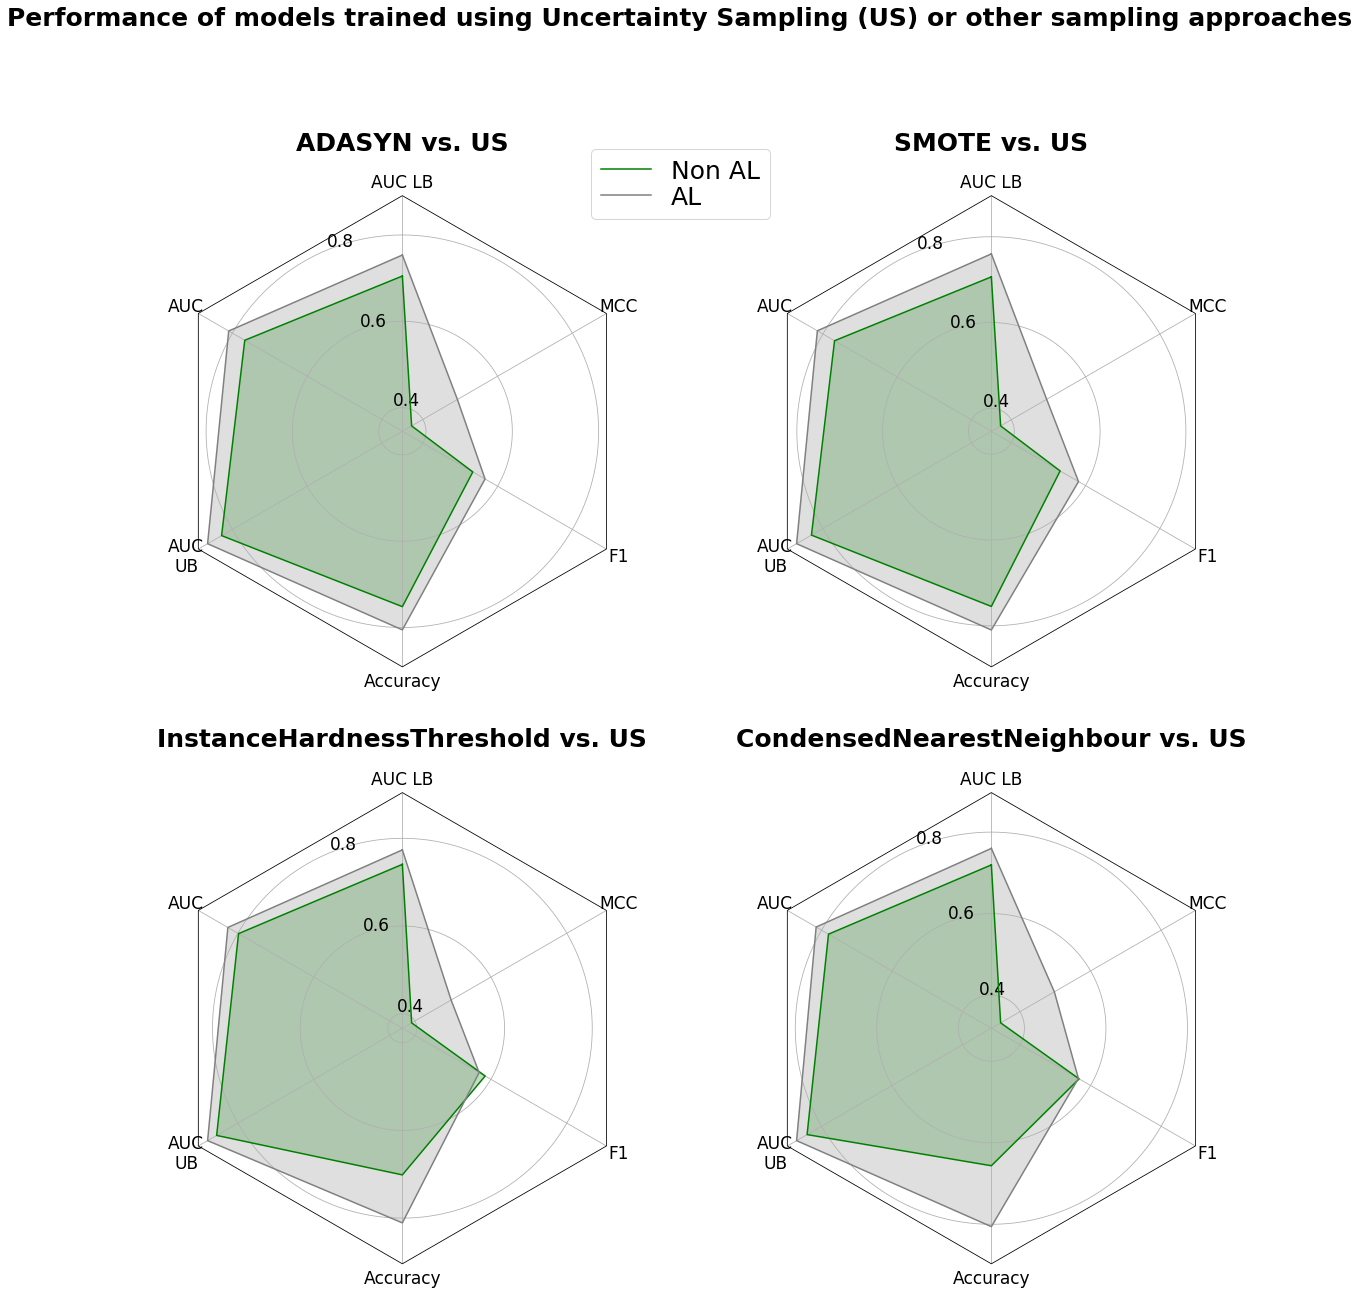
\includegraphics[keepaspectratio=true, scale=0.32]{images/sampling_imbalanced_learn.png}
    \caption{Performance of models trained using Uncertainty Sampling (US) or other sampling approaches}
    \label{fig:1}
\end{figure}

\begin{figure}
    \centering
    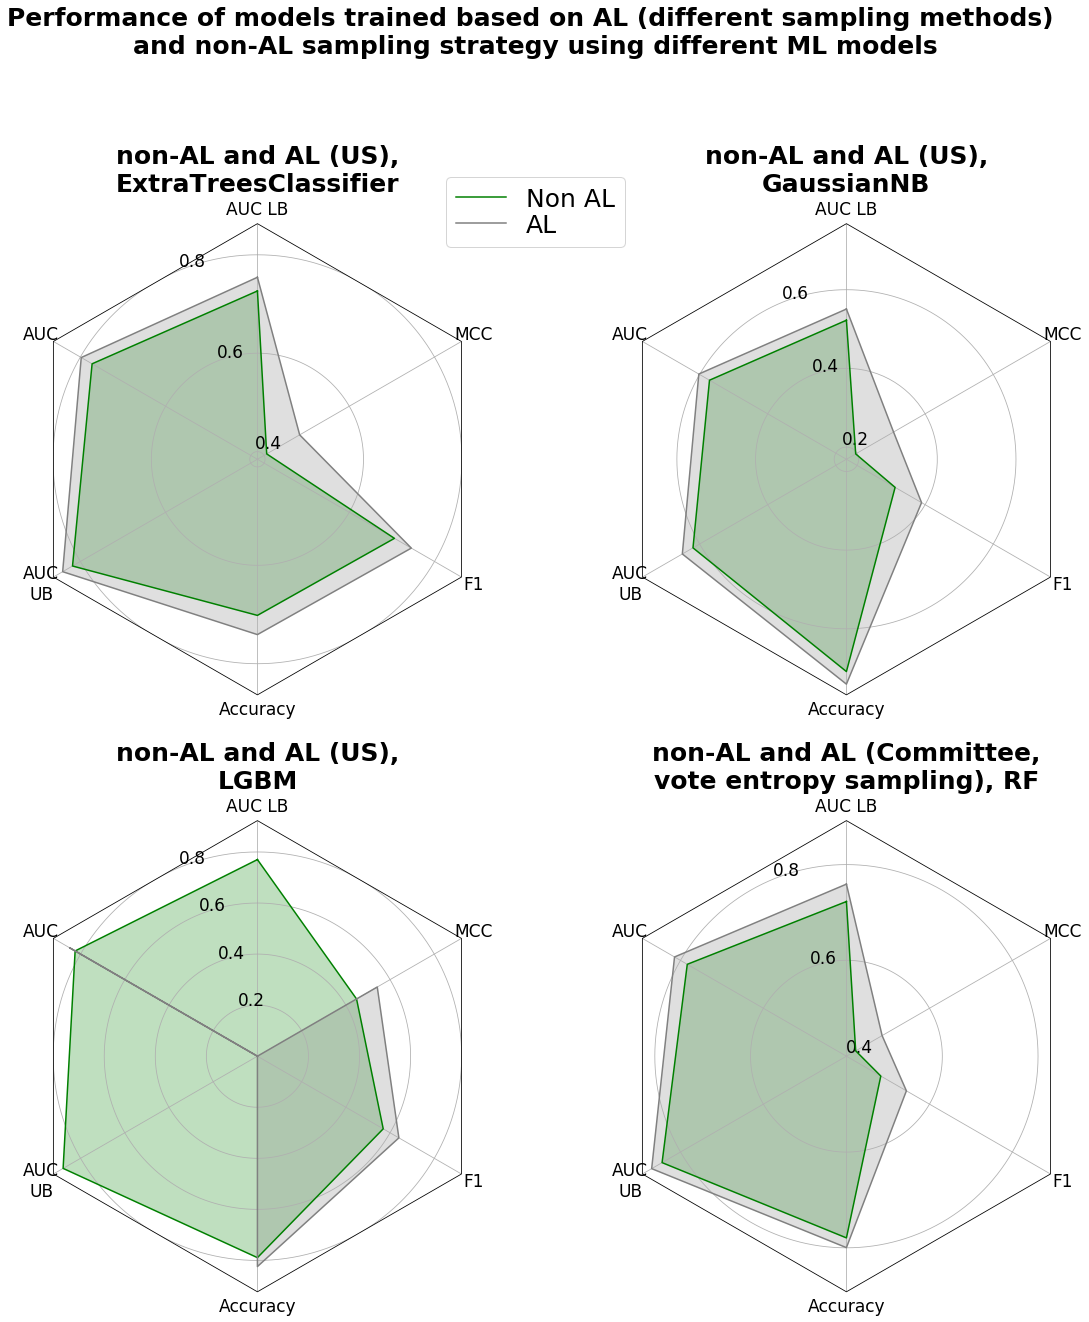
\includegraphics[keepaspectratio=true, scale=0.32]{images/models_and_sampling.png}
    \caption{Performance of models trained based on AL (different sampling methods) and non-AL sampling strategy using different ML models}
    \label{fig:2}
\end{figure}

\begin{figure}
    \centering
    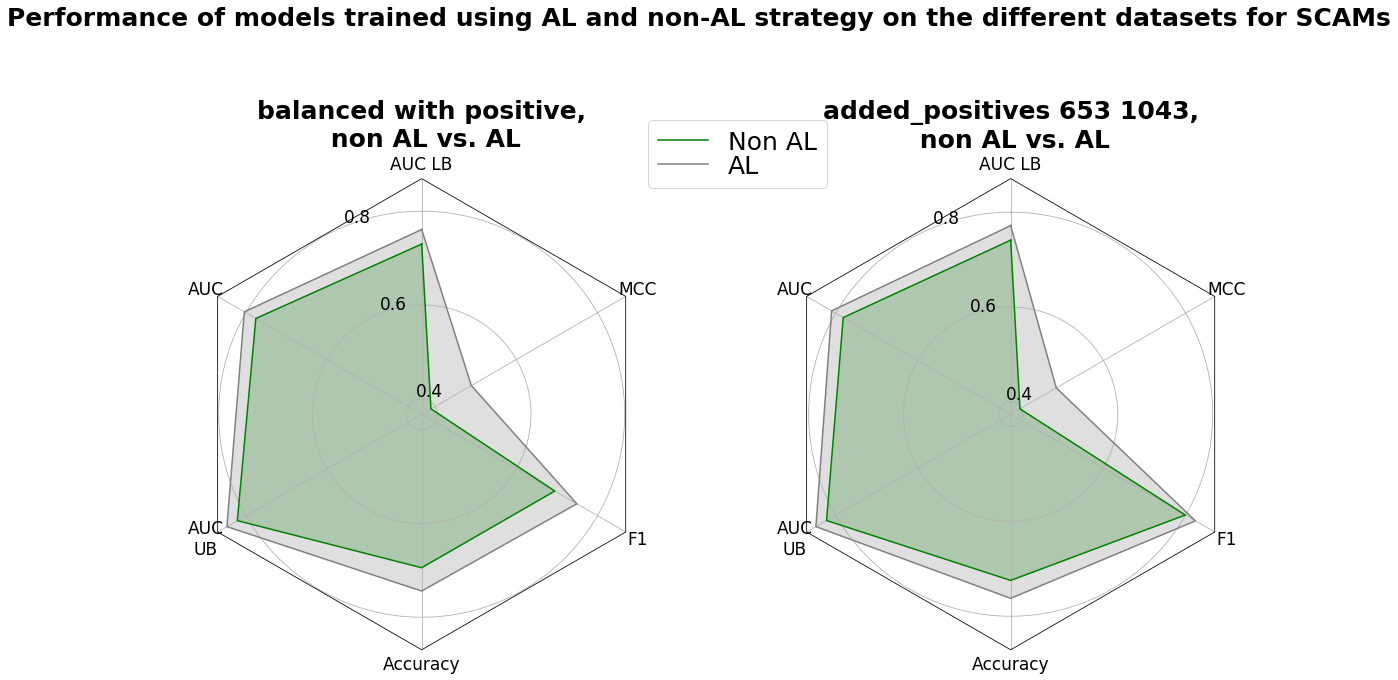
\includegraphics[keepaspectratio=true, scale=0.32]{images/different_data.png}
    \caption{Performance of models trained using AL and non-AL strategy on the different datasets for SCAMs}
    \label{fig:3}
\end{figure}


\begin{figure}
    \centering
    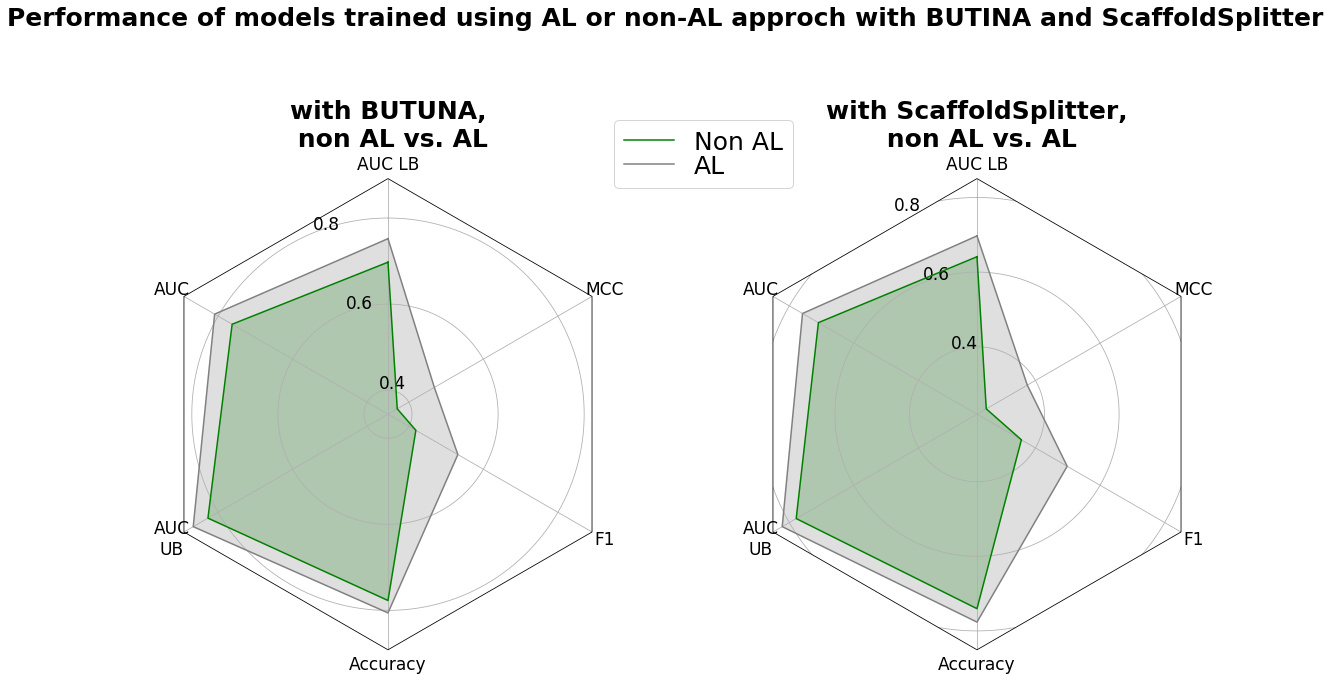
\includegraphics[keepaspectratio=true, scale=0.32]{images/splitters.png}
    \caption{Performance of models trained using AL and non-AL strategy with different splitters}
    \label{fig:3}
\end{figure}


\medskip

%Sets the bibliography style to UNSRT and imports the 
%bibliography file "samples.bib".
\bibliographystyle{unsrt}
\bibliography{sample}

\end{document}
